\documentclass{article}
\usepackage[utf8]{inputenc}
\usepackage{graphicx}

\title{Membuat Aplikasi Dengan Menggunakan Data Yang Telah Di Normalisasi}
\author{Helmi Azhar (1184013) }
\date{November 2019}

\begin{document}

\maketitle

\section{Oracle express}
\begin{enumerate}
\usepackage{Oracle Apex merupakan suatu aplikasi atau tools  untuk memudahkan apa yang kita butuhkan. Sesuai namanya, oracle express bila dipelajari lebih dalam banyak memberi kemudahan dalam melayanani kebutuhan user contohnya dalam pembuatan aplikasi sederhana,belajar function dan lain-lain. Oracle apex juga dapat mengembangkan aplikasi web desktop dan seluler, memvisualisasikan dan memelihara data basis data, dan meningkatkan keterampilan sql dan kemampuan basis data}
\end{enumerate}

\begin{enumerate}
    \usepackage{pada tugas kali ini saya akan membuat aplikasi di oracle express dengan menginput data dari excell yang telah di normalisasi dengan menginputkan data tabel dosen,tabel jadwal,tabel kuliah,tabel mahasiswa,dan tabel nilai.}
\end{enumerate}

\section{Langkah-langkah}
\begin{enumerate}
    \item sign in dengan akun masing-masing
    \begin{center}
        \centering
        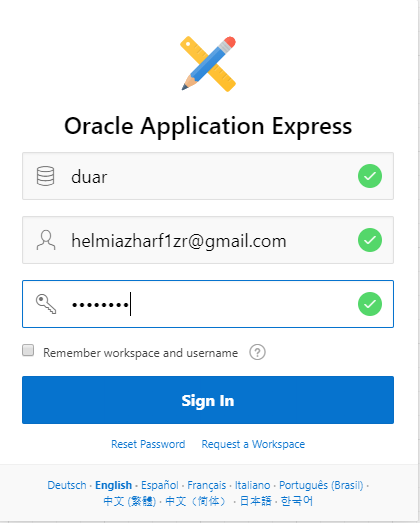
\includegraphics[scale=0.5]{figures/1.PNG}
        \caption{Caption}
        \label{fig:my_label}
    \end{center}

    \item setelah sign in pilih app builder
    \begin{center}
        \centering
        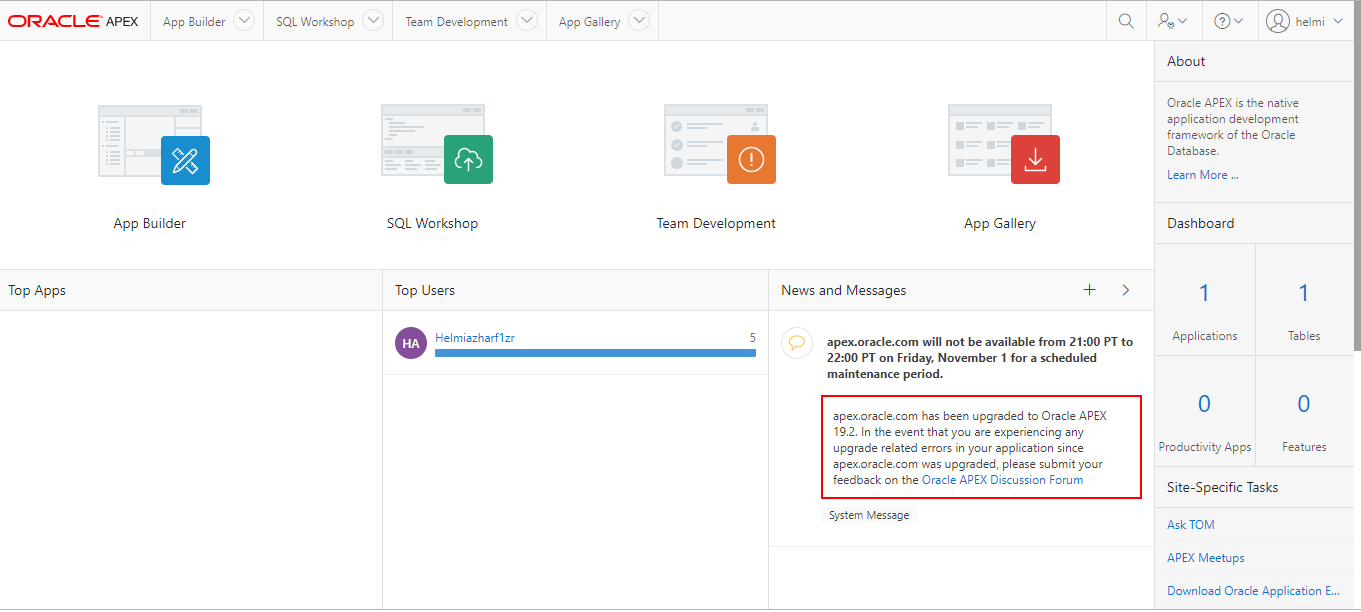
\includegraphics[scale=0.4]{figures/2.PNG}
        \caption{Caption}
        \label{fig:my_label}
    \end{center}

    \item buka create
    \begin{center}
        \centering
        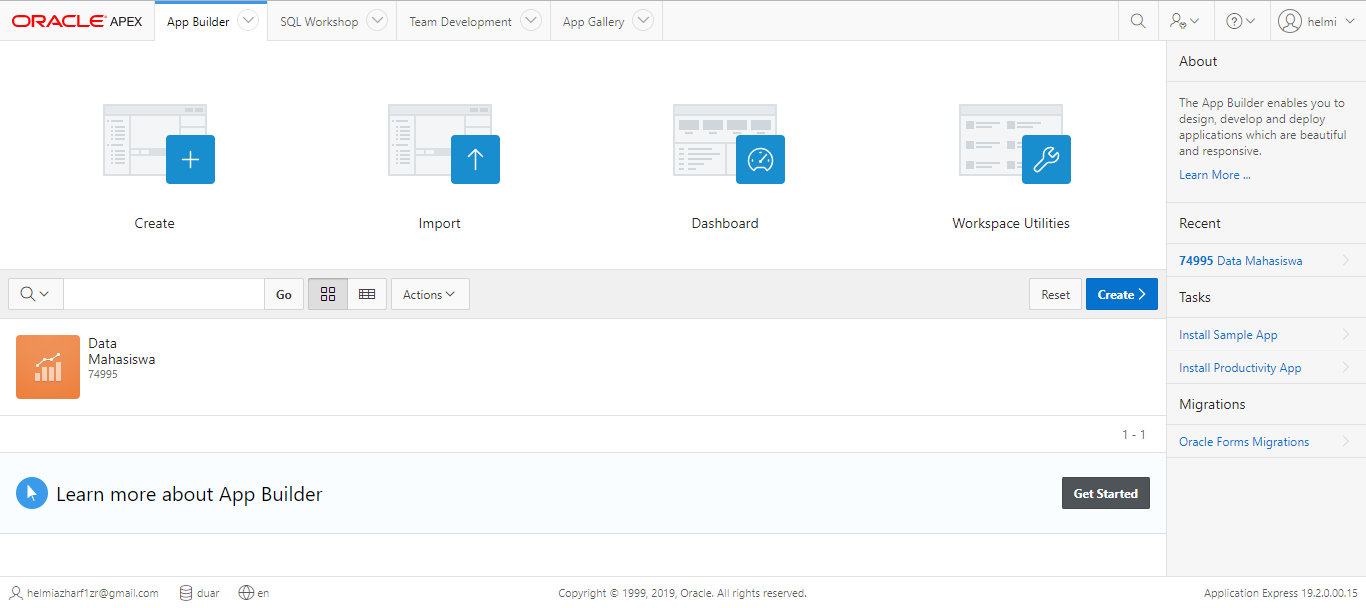
\includegraphics[scale=0.4]{figures/3.PNG}
        \caption{Caption}
        \label{fig:my_label}
    \end{center}

    \item lalu pilihm from a file
    \begin{center}
        \centering
        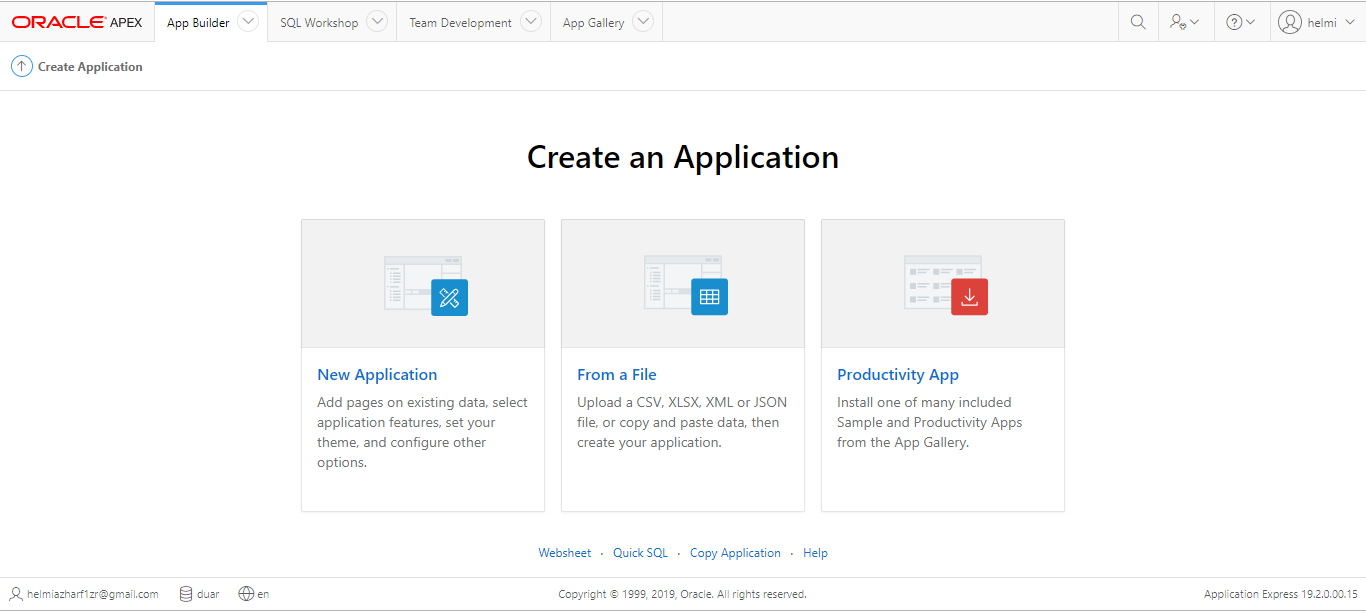
\includegraphics[scale=0.4]{figures/4.PNG}
        \caption{Caption}
        \label{fig:my_label}
    \end{center}

    \item pilih file tabel dosen,tabel jadwal,tabel kuliah,tabel mahasiswa,dan tabel nilai excel yang sudah di normalisasi lalu upload
    \begin{center}
        \centering
        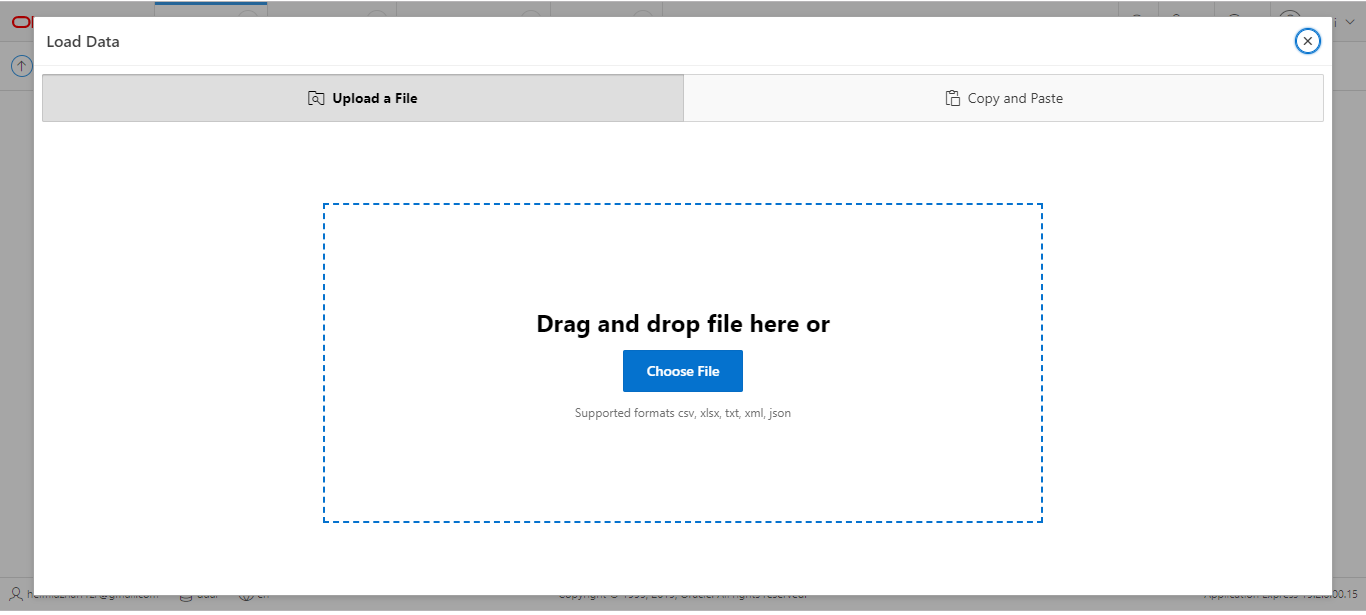
\includegraphics[scale=0.4]{figures/5.PNG}
        \caption{Caption}
        \label{fig:my_label}
    \end{center}
    
    \item Setelah di upload buat nama lalu load data
    \begin{center}
        \centering
        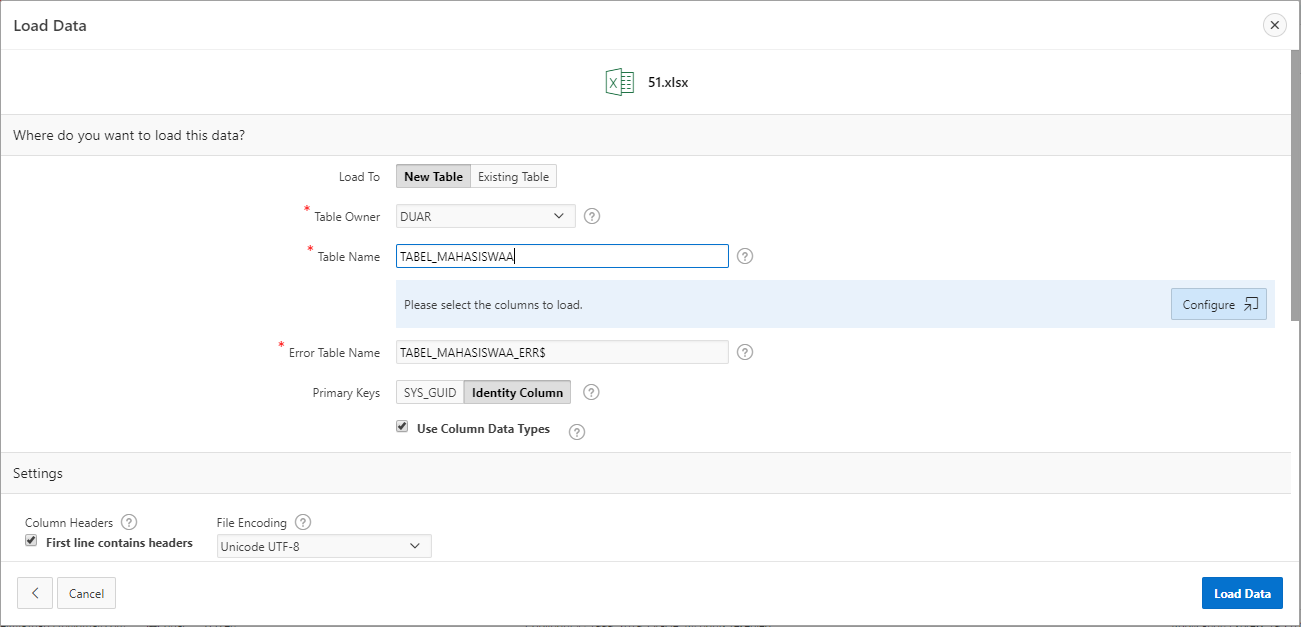
\includegraphics[scale=0.4]{figures/8.PNG}
        \caption{Caption}
        \label{fig:my_label}
    \end{center}
    
        \item Lalu pilih view table jangan dulu di create application
    \begin{center}
        \centering
        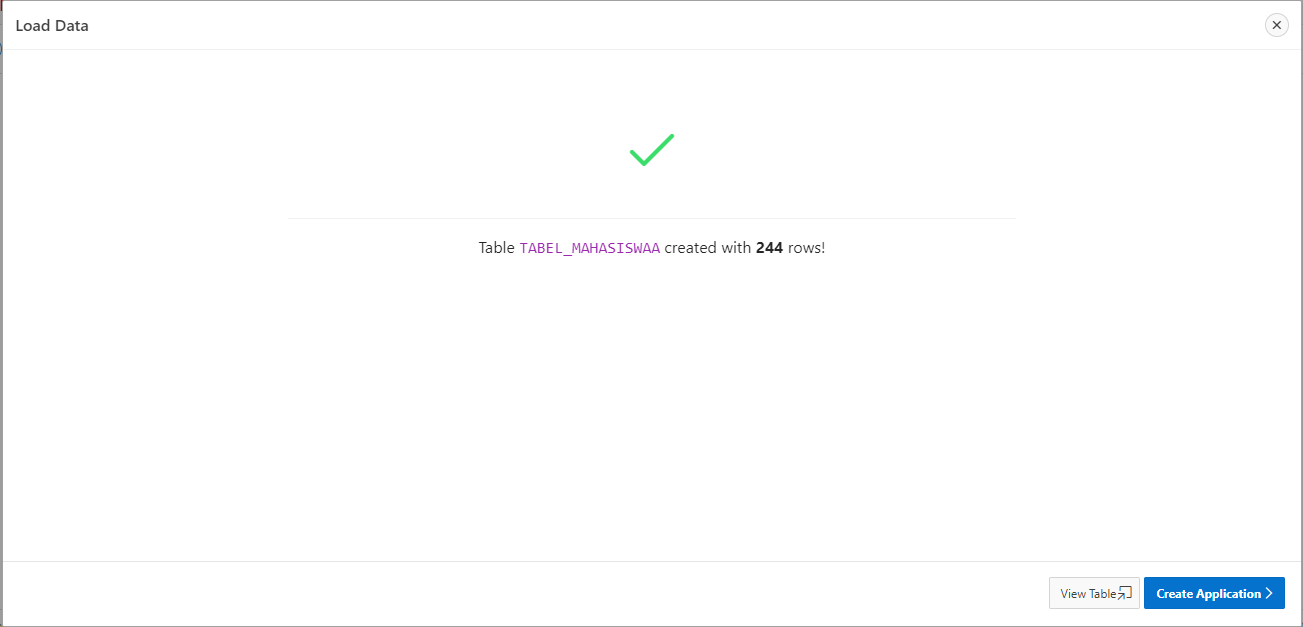
\includegraphics[scale=0.4]{figures/9.PNG}
        \caption{Caption}
        \label{fig:my_label}
    \end{center}
    
        \item Setelah itu buka masing masing tabel 
    \begin{center}
        \centering
        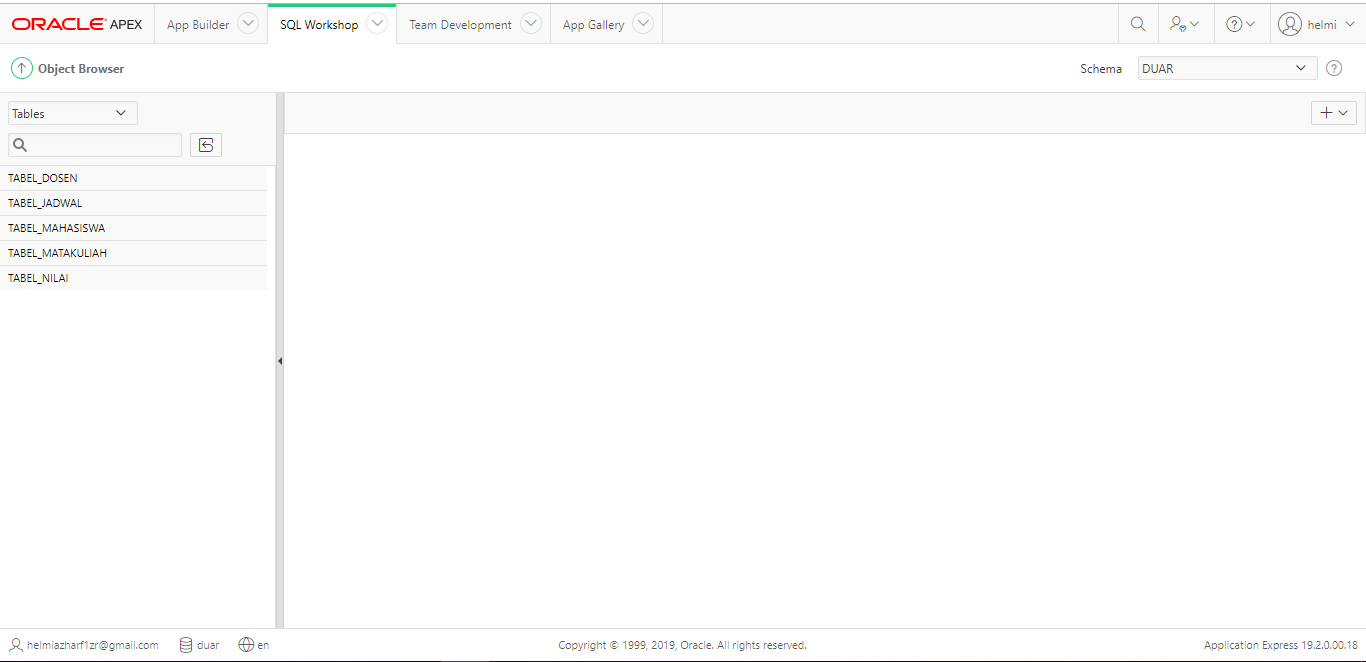
\includegraphics[scale=0.4]{figures/7.PNG}
        \caption{Caption}
        \label{fig:my_label}
    \end{center}

        \item karena oracle apex tidak bisa membaca primary key disetiap tabel maka oracle apex menambah id secara otomatis maka kita harus menghapus id tersebut dengan cara klik drop colomn dan pilih id lalu drop colomn
    \begin{center}
        \centering
        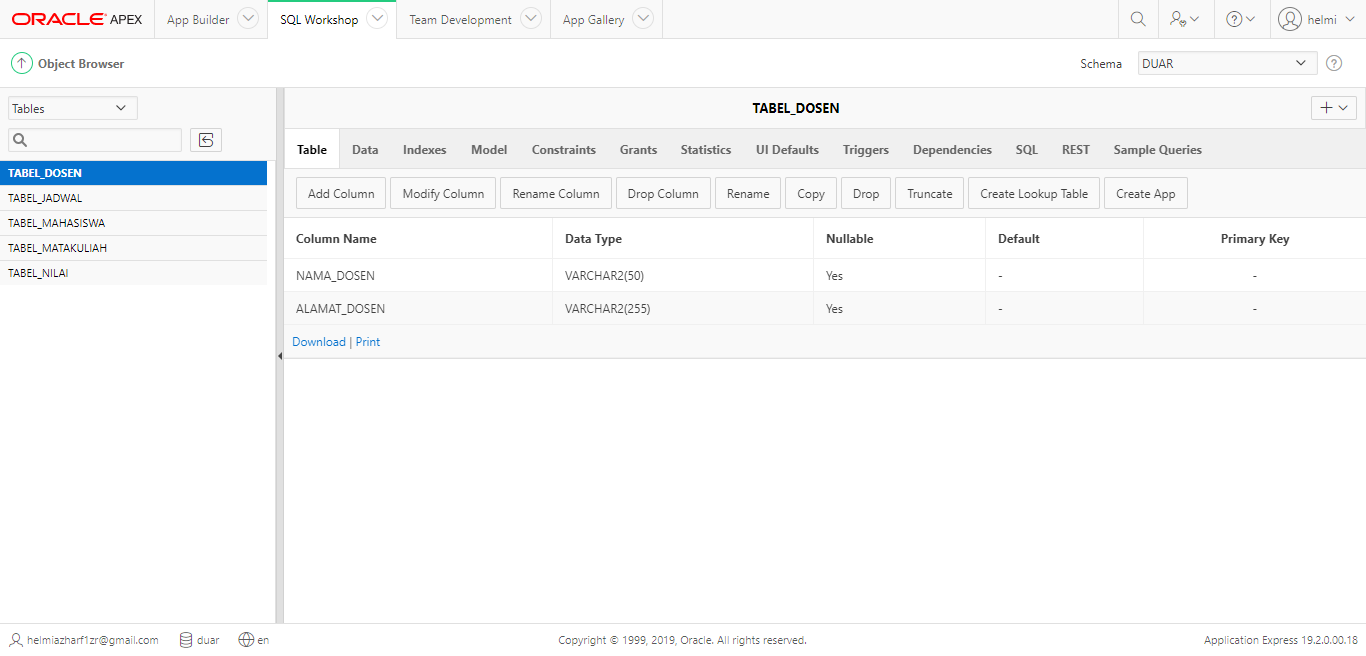
\includegraphics[scale=0.4]{figures/10.PNG}
        \caption{Caption}
        \label{fig:my_label}
    \end{center}
    
            \item Setelah itu buka masing masing tabel 
    \begin{center}
        \centering
        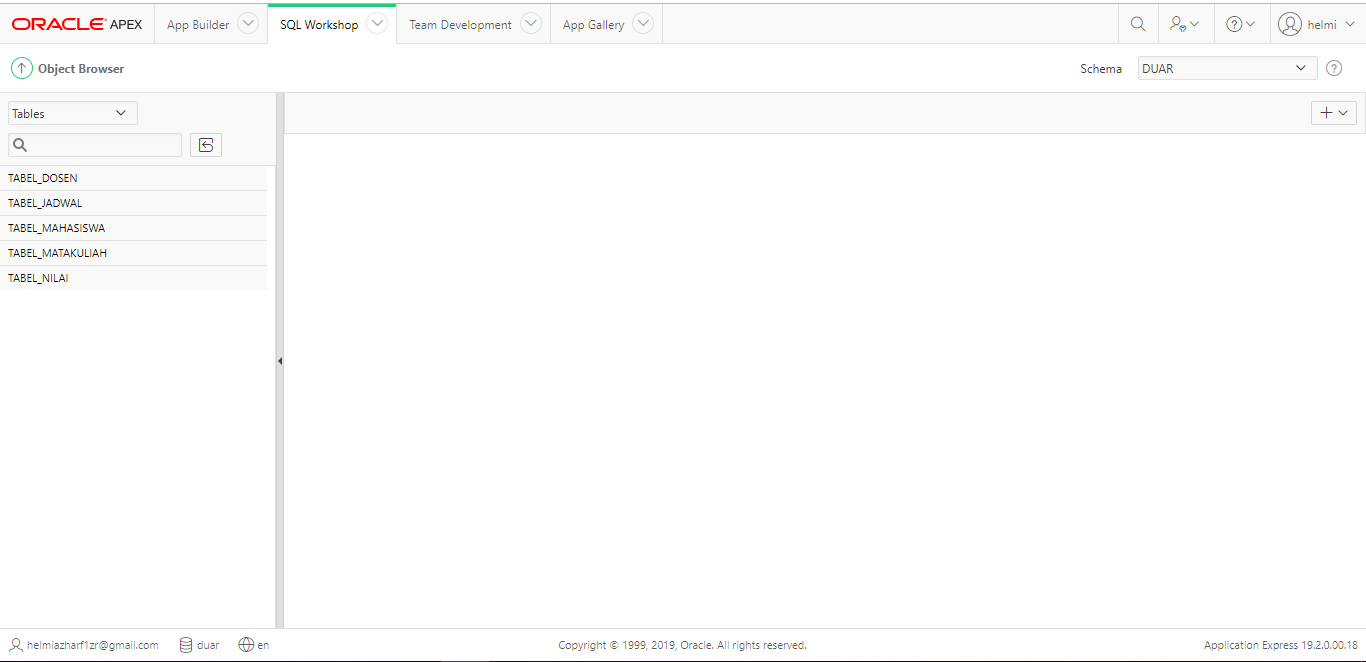
\includegraphics[scale=0.4]{figures/7.PNG}
        \caption{Caption}
        \label{fig:my_label}
    \end{center}
    
                \item Setelah itu buka SQL workshop lalu buka SQL commands dan masukan primary key untuk tabel mahasiswa,dosen,dan mata kuliah lalu run
    \begin{center}
        \centering
        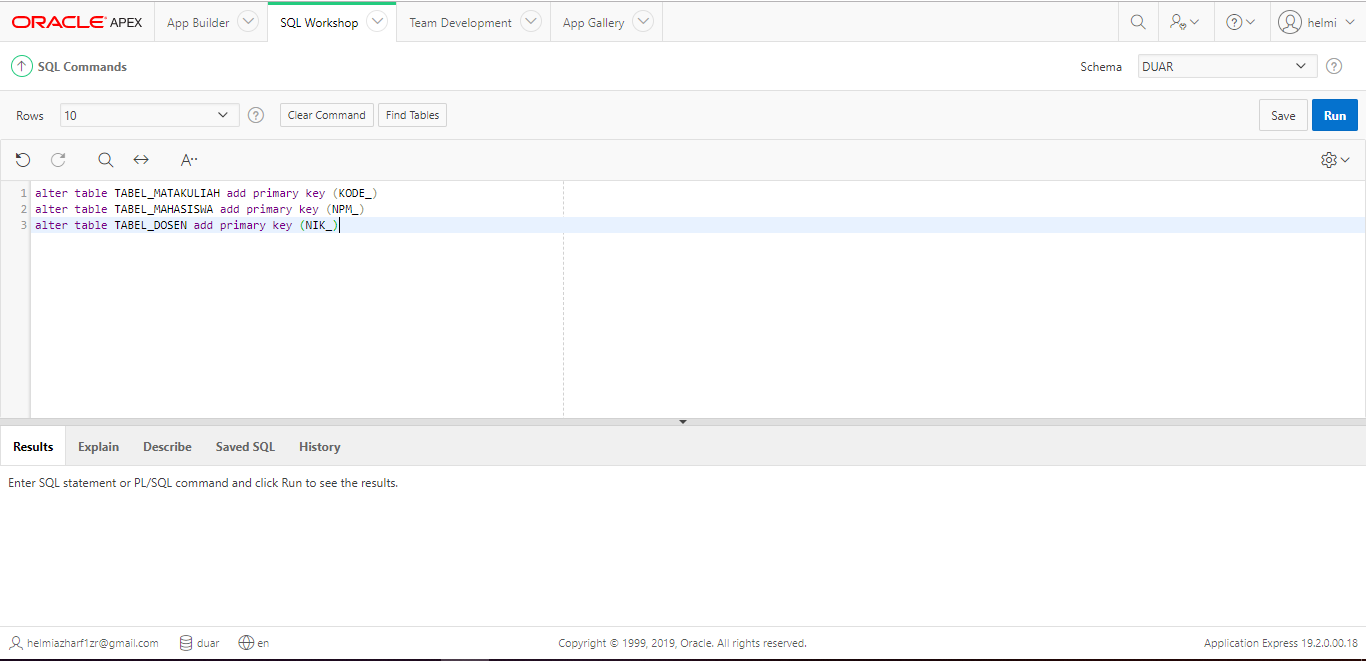
\includegraphics[scale=0.4]{figures/11.PNG}
        \caption{Caption}
        \label{fig:my_label}
    \end{center}
    
                    \item Setelah itu buka SQL workshop lalu buka SQL commands dan masukan foreign key untuk tabel dosen dan tabel mata kuliah dalam tabel jadwal
    \begin{center}
        \centering
        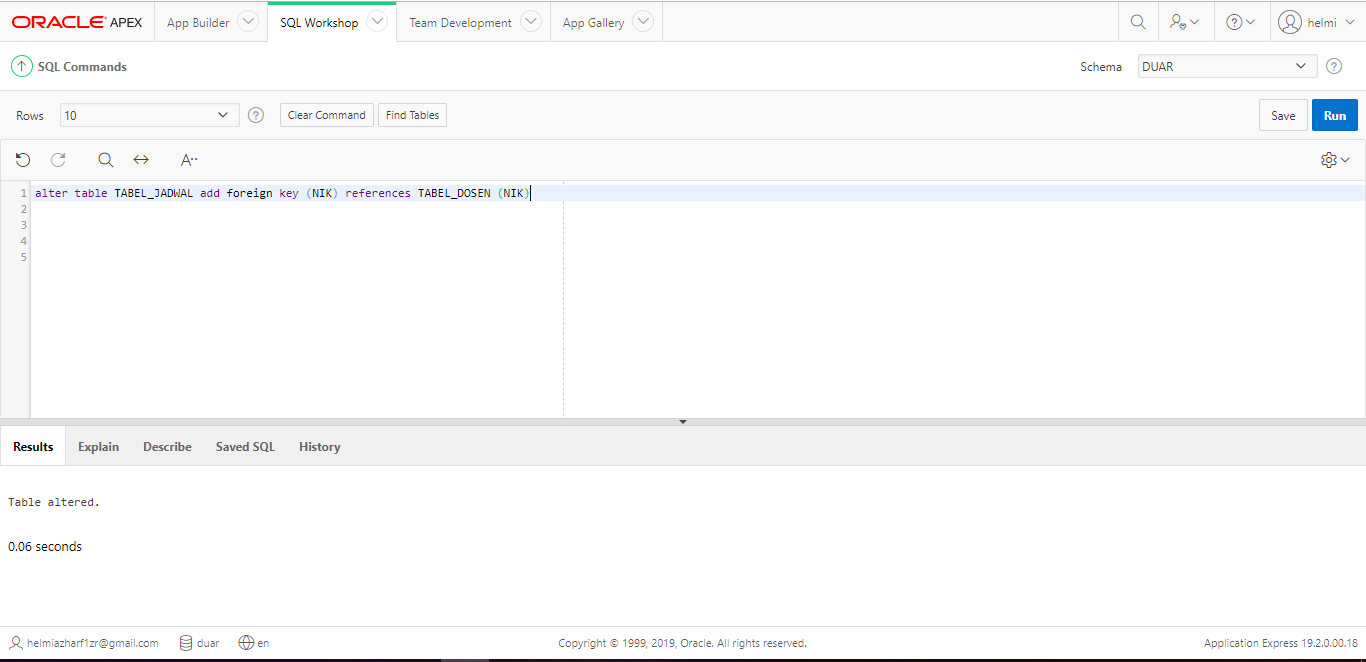
\includegraphics[scale=0.4]{figures/12.PNG}
        \caption{Caption}
        \label{fig:my_label}
    \end{center}
    
                        \item Setelah itu buka SQL workshop lalu buka SQL commands dan masukan foreign key untuk tabel dosen dan tabel mata kuliah dalam tabel jadwal
    \begin{center}
        \centering
        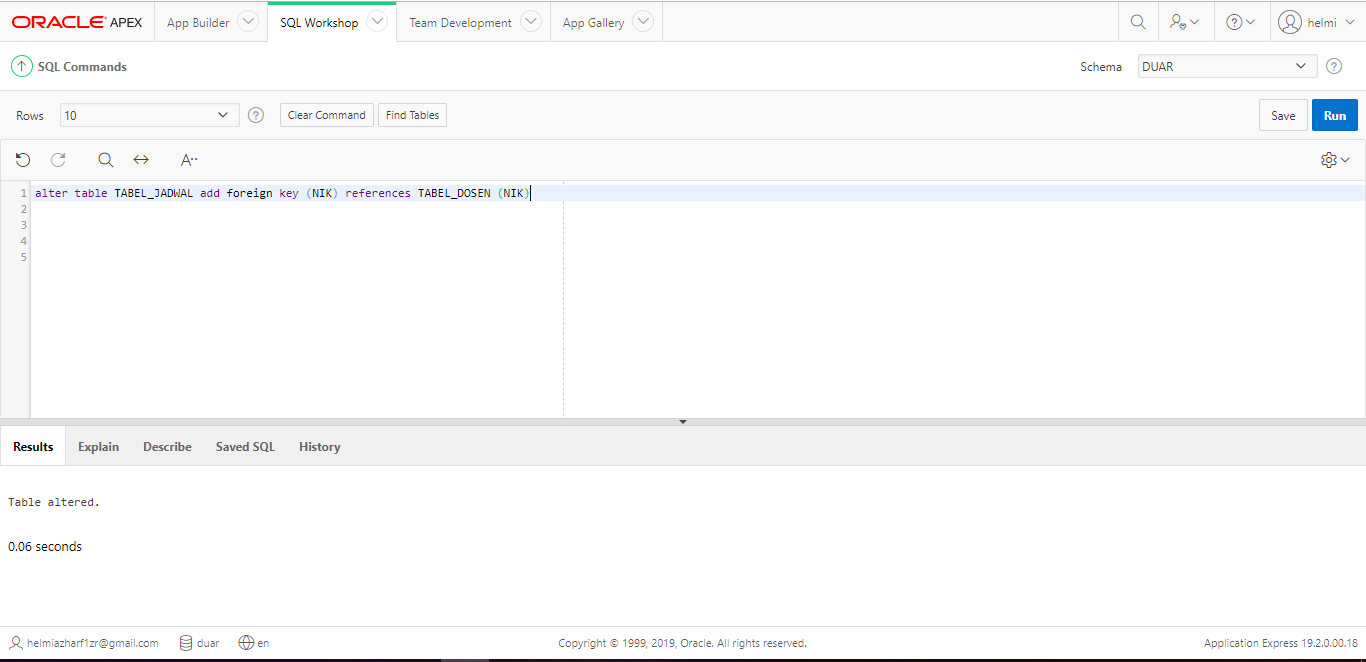
\includegraphics[scale=0.4]{figures/12.PNG}
        \caption{Caption}
        \label{fig:my_label}
    \end{center}
    
                            \item buka new application
    \begin{center}
        \centering
        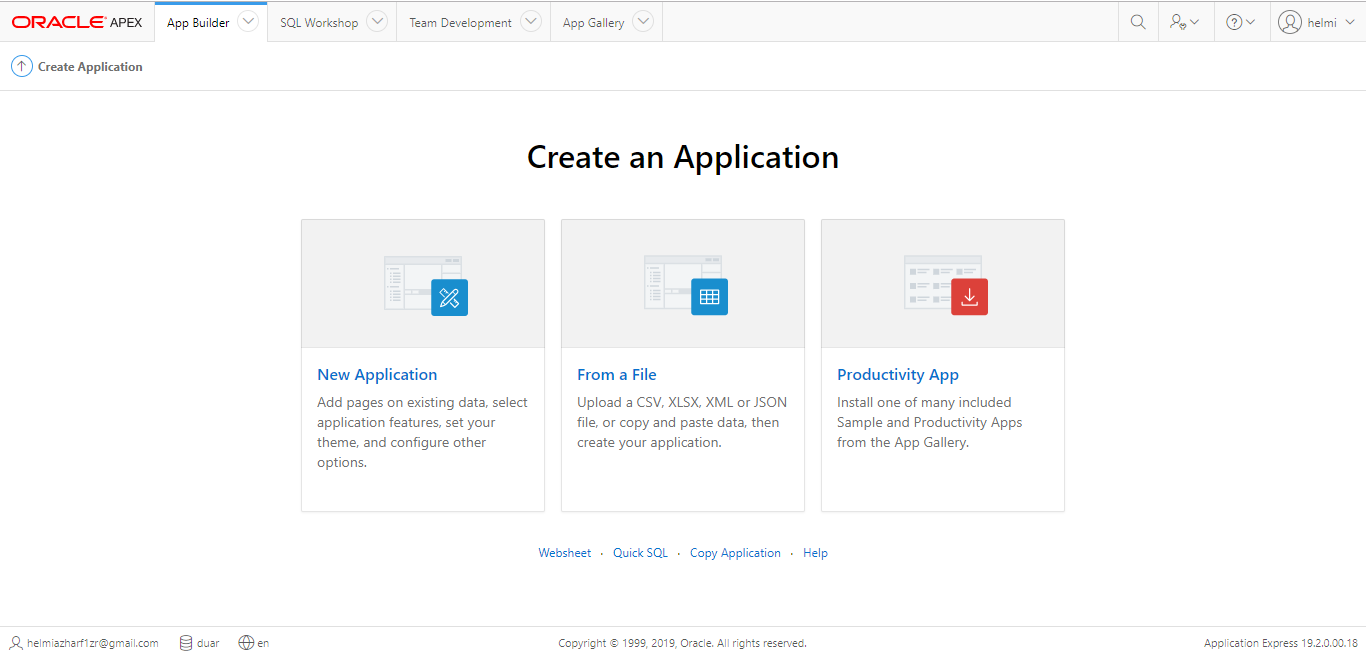
\includegraphics[scale=0.4]{figures/13.PNG}
        \caption{Caption}
        \label{fig:my_label}
    \end{center}
    
                               \item isi nama aplikasi lalu pilih add page dan pilih interactive report dan masukan satu per satu tabelnya
    \begin{center}
        \centering
        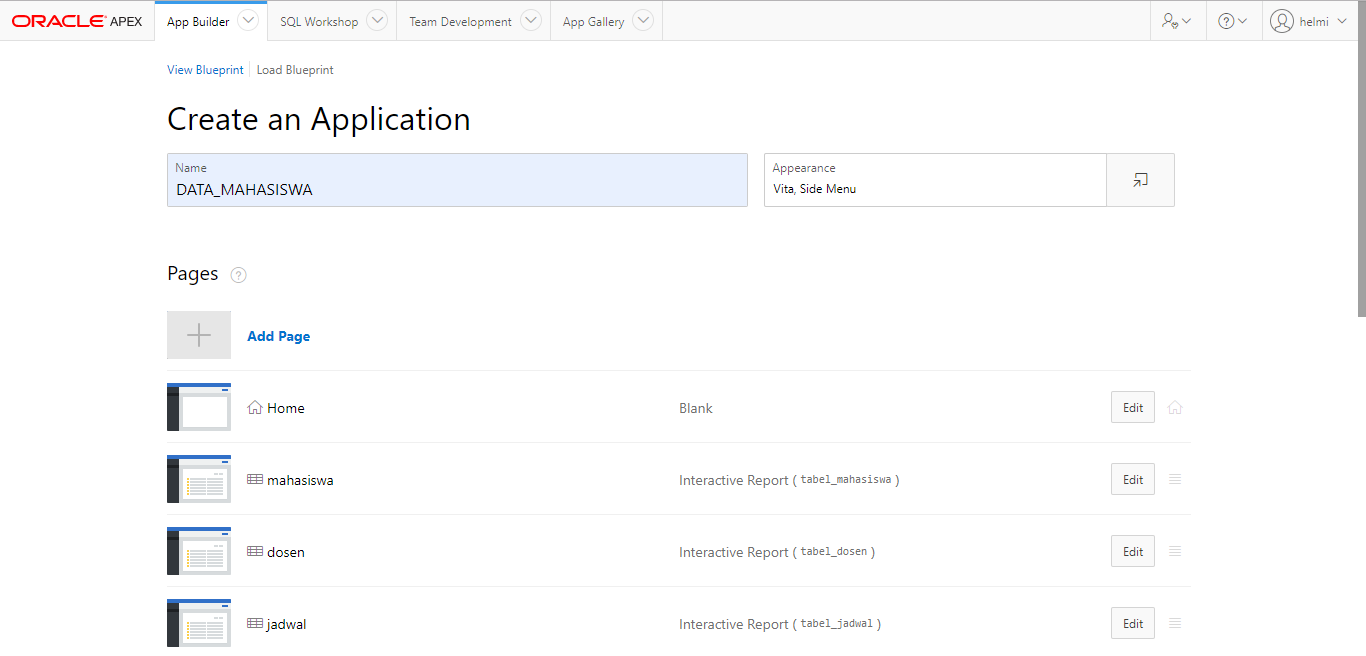
\includegraphics[scale=0.4]{figures/14.PNG}
        \caption{Caption}
        \label{fig:my_label}
    \end{center}
    
                                   \item lalu create application
    \begin{center}
        \centering
        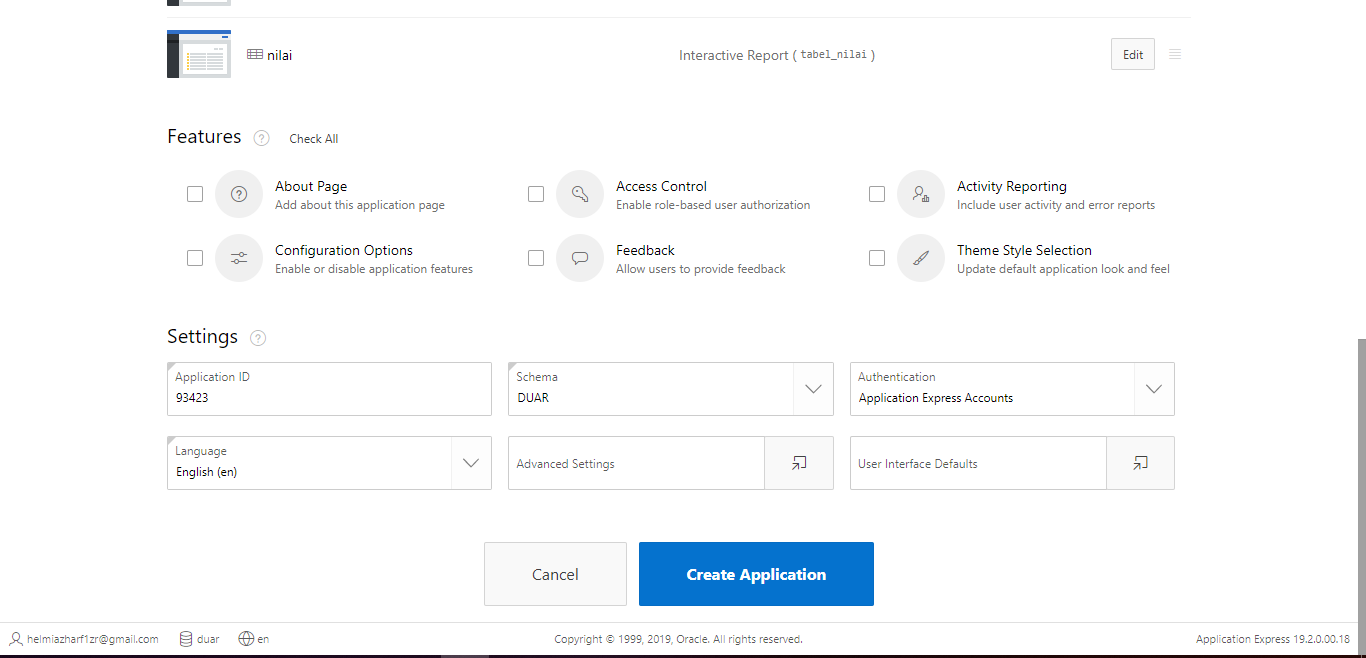
\includegraphics[scale=0.4]{figures/15.PNG}
        \caption{Caption}
        \label{fig:my_label}
    \end{center}
                                    \item pilih run application
    \begin{center}
        \centering
        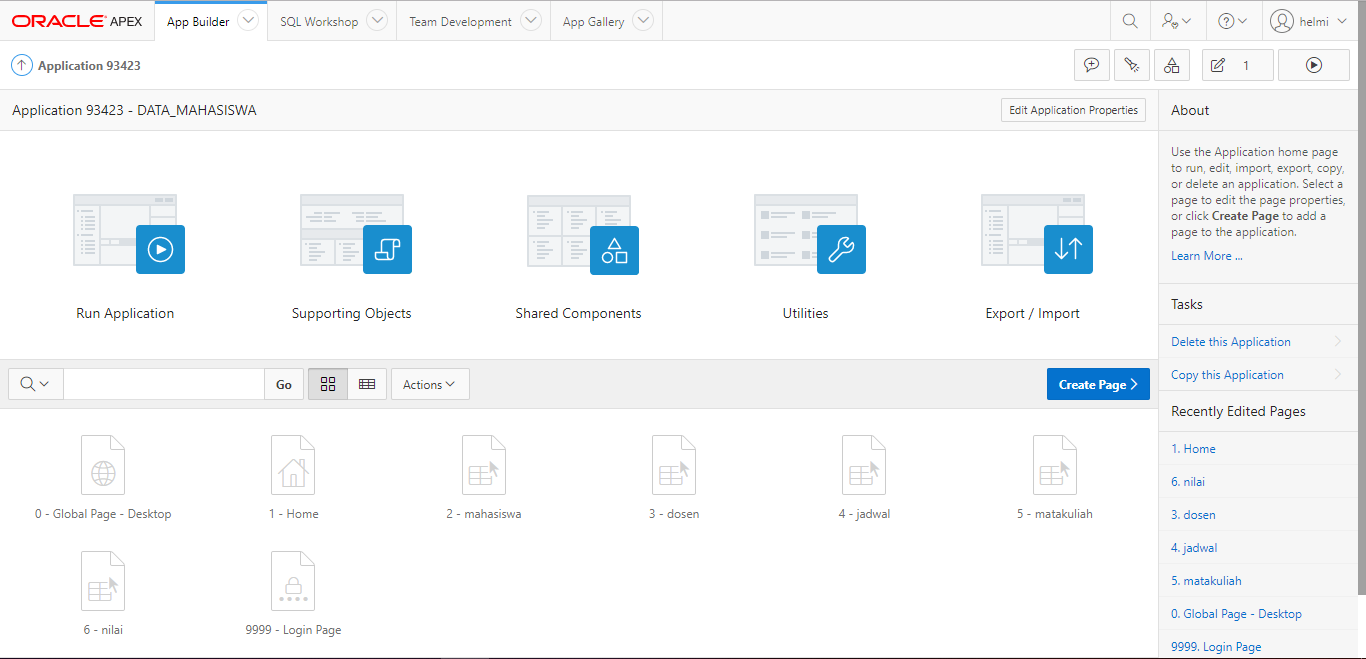
\includegraphics[scale=0.4]{figures/16.PNG}
        \caption{Caption}
        \label{fig:my_label}
    \end{center}
    
                                        \item sign in
    \begin{center}
        \centering
        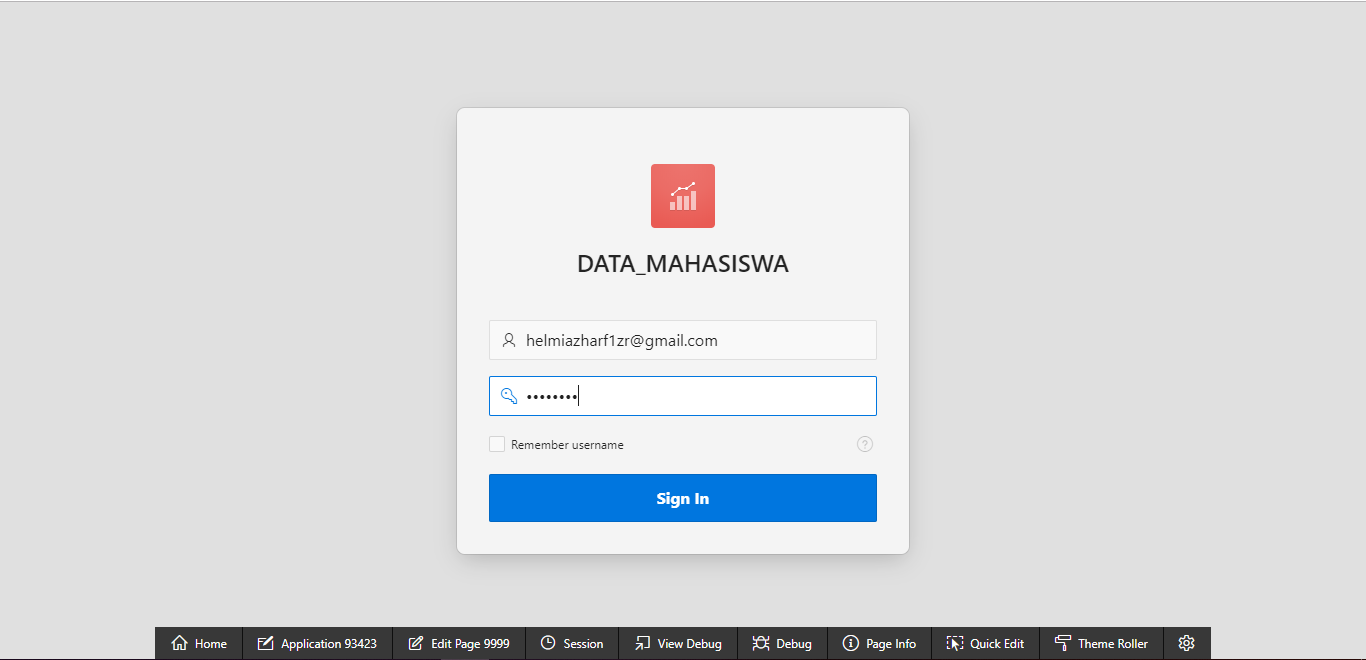
\includegraphics[scale=0.4]{figures/17.PNG}
        \caption{Caption}
        \label{fig:my_label}
    \end{center}
    
                                            \item aplikasi selesai
    \begin{center}
        \centering
        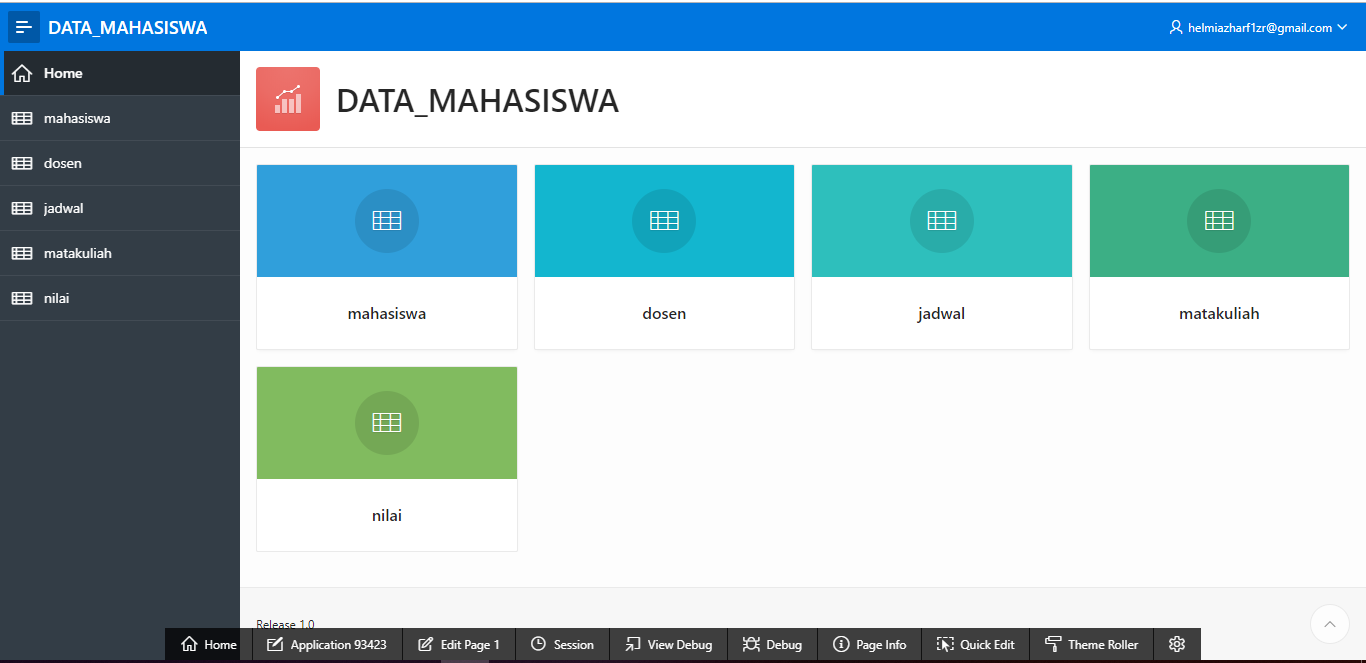
\includegraphics[scale=0.4]{figures/18.PNG}
        \caption{Caption}
        \label{fig:my_label}
    \end{center}
    
    \end{enumerate}
    
\section{Data Saya}
\begin{enumerate}
    \item Link= https://apex.oracle.com/pls/apex/f?p=93423:LOGIN\textunderscore DESKTOP:706963636601732:::::
    \item workspace = "duar"
    \item username = "helmiazharf1zr@gmail.com"
    \item password = "password"
\end{enumerate}

    
\end{document}